% !TEX root = thesis.tex

\chapter{The Importance of Hotel Recognition}
\label{ch:1}

In recent years, the number of images of victims of human trafficking available online has grown at an alarming rate~\cite{bouche2015report,ncmecAmicusBrief}. Whether used
for advertising or exchanged among criminal networks, these photographs can serve as visual evidence of where the victim was trafficked. Such images are often captured in hotel rooms. Identifying the hotels in these photographs (Figure~\ref{fig:frontPage}) to understand where a victim was gives insight into trafficking operations, which is a a top priority for law enforcement~\cite{nationalStrategy}.

\begin{figure}
    \centering
    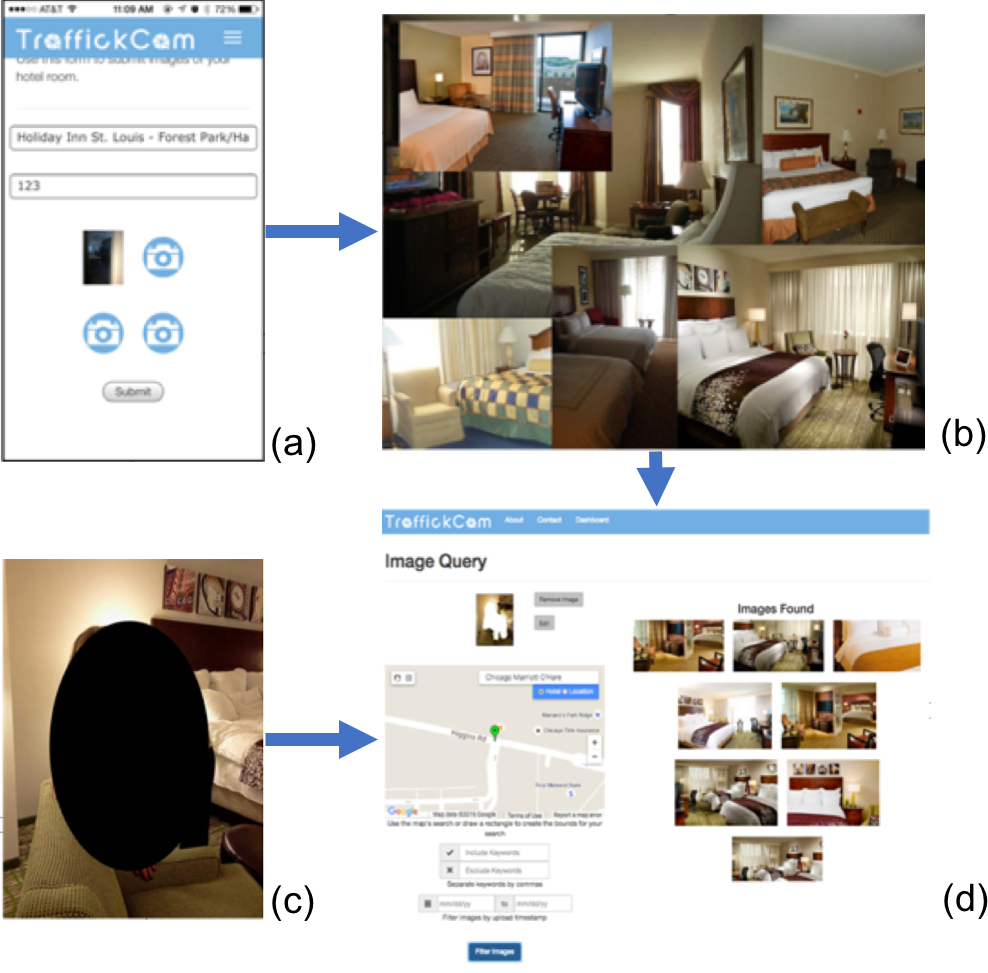
\includegraphics[width=.9\columnwidth]{figures/front_page_figure.png}
    \caption{The Hotels-50K dataset supports the development of hotel recognition algorithms to help in investigations of human trafficking by identifying the hotel where a picture was taken.}
    \label{fig:frontPage}
\end{figure}

Figure~\ref{fig:queries} gives a few example of law enforcement queries.  Often the region of the images containing the victim is
masked for privacy and legal reasons.  Algorithms for recognition in this context must be robust to large occlusions, varying lighting conditions, and the unique perspectives of a hotel room.
